\chapter{Technical Design}
\label{chap:technical}

This chapter includes the technical details of \emph{Dockit League}'s various components as well as a combination of design and technical information on all of the docking kits.  

\section{Architectures in Unity}
When developing in Unity, or any existing game engine, the engine will heavily influence the basic architecture of the solution. Therefore, a basic understanding of the Unity engine can give a better understanding of the architecture in our solution. This section will include a basic description of the core concepts and terminology in Unity.

\subsection{General overview}
Unity is an component based engine, which means it moves away from the traditional OOP design with complex hierarchies. The traditional use of monolithic class hierarchies limits our design, and may force us to inherit from classes we don't really require. It makes it difficult to extend functionality, as it may affect objects further down the hierarchy. However, using a component design allows isolating the various features in a single compact service. In that way the components are decoupled, and functions independently of each other. To maintain the components a container/hub is needed. When designing an object, you can then add whichever component required to the container, giving us a lot of flexibility.~\cite{gameEngineArch}

In Unity every object in the game will be a \emph{GameObject}, which is Unity's container for components. Custom scripts can be placed on these \emph{GameObjects} if they derive from the built-in class named \emph{MonoBehaviour}. This is a necessary step to connect the script to the internal Unity pipeline, and will let Unity handle the component management.~\cite{unityScriptManual} You can store a particular GameObject setup in something called a \emph{prefab}, which makes it easy to reference this object. Unity also has a container for \emph{GameObjects} called scenes. These are used to separate different parts of the game, different levels for instance.

\subsection{Networking overview}
Unity's networking system is referred to as their High Level API (HLAPI). This gives developers a way to access networking functionality without dealing with low level networking. The lower transport layer supports any kind of network topology, but the HLAPI uses a server authoritative system, and it's what our solution is built with.

The standard base class for scripts is \emph{MonoBehaviour}, however, for networked scripts the base class is \emph{NetworkBehaviour}. This derives from \emph{MonoBehaviour}, thus has all the same functionality, but will in addition be included in the networking system. \emph{NetworkBehaviours} may have member variables that takes advantage of the \emph{SyncVar} attribute. This is a way for the server to synchronize the state to each remote client. However, the data types are restricted to basic data types (byte, int, float, string, etc), built-in Unity math types (Vector3, Quaternion, etc), and structs containing the previous two.

The networking system has three different ways of calling remote actions across the network by adding custom attributes to a function. This means the function will be invoked through the HLAPI. \emph{Command} is called by a client with authority and will run on the server. \emph{ClientRpc} is called by the server call and will run on every client. \emph{TargetRpc} is called by the server and will run on a specific client. The restrictions to the available parameter data type is the same as \emph{SyncVars}.~\cite{unityUNETManual}

\section{General architecture}

\subsection{Unity's example project}
When it was time to wrap the parts of the game into a playable state with networked menu, lobbies and scene management a few parts in our solution were heavily based on a reference project provided by Unity themselves~\cite{unityTanksProject}. As these parts of the solution weren't our focus, and time was restricting, this was a way to actually get a playable prototype ready on time. The things needed were extracted from that asset, and tweaked to fit our use.

\subsection{GameManager}
The \emph{GameManager} exists in every scene, and after we integrated Unity's example project it contains mostly code from that solution. The script also contains references to all of the Docking Kit prefabs and the player UI which includes both the in-game and pause menus. 

\subsection{SpawnableFactory}
The \emph{SpawnableFactory} handles all the spawning (instantiation) of GameObjects in the solution. It contains a list of all spawned objects, which makes it easy for the game to clean-up spawned objects when a round ends for instance. The majority of objects spawned derive from the \emph{SpawnableObject} class, which handles the ownership related data. This includes the player owning the object, as well as the associated team ID. The only other type of object spawned is the Docking Kit Pickup. The pickup doesn't need the ownership data, which is why it's not a \emph{SpawnableObject}, but it basically has the same functionality in the SpawnableFactory. By collecting all the spawning in one place, it makes the handling easier.

\subsection{In-game UI}
The \emph{PlayerUIHandler} component handles the UI elements for the player. It has functionality for updating the health elements, ability elements, and status elements. The handler receives calls whenever a Docking Kit changes, extracts the ability information from the \emph{DockingKit} component, and delegates them to the \emph{AbilityUI} classes, which handles the individual abilities. The \emph{StatusUI} prefab is instantiated on the status bars for every status effect added to the player. This component displays the information regarding the individual effect, like duration and effect icon. This utilizes the Unity UI \emph{Grid Layout Group} component, to automatically format the UI elements instantiated, meaning the only thing necessary for the status effect to appear correctly is to spawn the object as a child of that layout group.

\section{Player architecture}

\paragraph{NetworkPlayer}
The \emph{NetworkPlayer} component is heavily based on the solution in the Unity example project.~\cite{unityTanksProject} And as such, won't be covered much here. However, in short, this component is not destroyed in between scenes, and handles the overall networking of a player both in the lobby and in-game.
\paragraph{LobbyPlayer}
This is the player representation in the lobby, and is also heavily based on the example project.

\subsection{Player}
The \emph{Player} component has parts that are based on the Unity example project, and part our own solution. This component is the player representation in the actual game. Our solution have three \emph{TargetRpcs} for adding force to the player, why this is necessary is discussed further in Section~\ref{sec:conForce}. These three functions are all different ways to add force to the player. They all take a parameter determining the strength of the force added, but the direction calculation differs. The first calculates the direction from the player position towards the given position. The second calculates from the given position towards the player position. The third uses a separate force function to add explosion force, and simply takes the explosion force and radius as parameters, along with the explosion position.
    
\subsection{Input}
The \emph{PlayerInput} component handles the input for each player, since this only happens locally it is a standard \emph{MonoBehaviour}. In addition to handling the input, it also does the actual movement for the player. This class needs to restrict certain types of inputs: movement, rotation, abilities, docking, and interactions, but a simple on/off solution would not work in our scenario. The restriction could come from different sources with different lengths, therefore the source applying the initial restriction might not be the one who should remove it, since other sources might arrive in the meantime and still want to apply the restriction. The solution to this is a simple stack, in which the sources simply add a count initially, and remove one when ending. When the count is 0 we know no one is applying a restriction, and the player is free to use that input type. Figure \ref{fig:inputRestrictionStack} shows an example of how the movement stack changes over time when a stun and root is applied and removed at different times, thus restricting the movement input.

\begin{figure}[htbp]
  \centering
  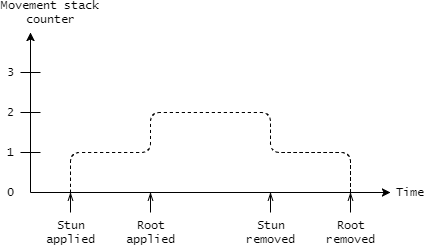
\includegraphics[width=.8\textwidth]{images/MovementStackCounter}
  \caption[Diagram showing the input restriction stack]{An example of how the input restriction stack works.}
  \label{fig:inputRestrictionStack}
\end{figure}
 


This component also handles interactable objects by keeping a reference to any object that implements the \emph{IInteractable} interface through \emph{OnTriggerEnter}. The interface function should be called on the server, to make sure only one player interacts with it at a time. This is handled through the \emph{Player} component with a command called by the \emph{PlayerInput} component, since the input component isn't networked.

\subsection{Field of View}
\label{sec:fieldOfView}
The basic implementation of the \emph{FieldOfView} component consists of creating the view mesh by casting rays from the player position with a certain angle step between, and then use the stencil buffer to only draw pixels covered by this mesh. The base implementation is not our work.~\cite{fieldOfViewGitHub}
Our additions to this implementation are functions for smoothly changing the view angle and view radius. This is handled by \emph{Coroutines} in the \emph{FieldOfView} component as seen here. The coroutine could been used as separate update loops, that runs and interpolates the value until it's at the target value, and then remove itself. The initialization of the angle coroutine can be seen in Listing~\ref{listing:setViewAngle}.

\begin{listing}[htb]
\begin{minted}[fontsize=\footnotesize]{csharp}
public void SetViewAngle(float newAngle, float speed) {
    if(angleCoroutine != null) {
        StopCoroutine(angleCoroutine);
    }
    angleCoroutine = StartCoroutine(ViewAngleLerp(newAngle, speed));
}
\end{minted}
\caption[Starting the angle coroutine]{Code snippet for starting the angle coroutine.}
\label{listing:setViewAngle}
\end{listing}

Keeping a reference to the started coroutine is necessary to prevent starting multiple coroutines, that all try to change the angle. In the case where multiple coroutines try to change the angle in opposite directions the loops could be stuck forever. By stopping any currently running routine before starting the new one there's always only one running, which will only move the current angle to the target angle with the speed given.
    
\subsection{Health and currency}
\paragraph{Player Health}
The \emph{PlayerHealth} component handles the functionality related to the player health, and is what other components use to apply damage to a player. It takes advantage of the \emph{SyncVar} functionality to synchronize the health across all clients, allowing the script to display the correct health color indicator for each player. Whenever damage is taken it will display a damage flash for every client, and update the UI for the local player. In addition to taking the damage, the source player of the damage will be stored. This allows the component keeping track of the score to extract which player got the killing blow to a player.

\paragraph{Currency}
The \emph{PlayerCurrency} component works very much like the \emph{PlayerHealth} component, so we grouped them together in this section. It uses a \emph{SyncVarHook} to keep the currency value synchronized between the server and the client. When the currency is changed by the server, the \emph{SyncVarHook} will check the difference between old and new currency and tells the \emph{PlayerUIHandler} to update the UI to the new value. When the \emph{PlayerUIHandler} updates the currency, it will also play an animation showing the difference being added or subtracted, as seen in Figure~\ref{fig:addCurrency}.

\begin{figure}[tbph]
  \centering
  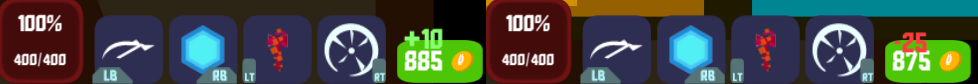
\includegraphics[width=\textwidth]{images/CurrencyChange}
  \caption[Example adding and subtracting currency]{Showing clearly when currency is added or removed}
  \label{fig:addCurrency}
\end{figure}


\subsection{Player Status}
The \emph{PlayerStatus} component handles the modifier instances and status effects applied to the player. Modifiers are applied on the server, which then synchronizes these out to every client. The instances of a modifier are split up in two: \emph{ModifierInstanceServer} and \emph{ModifierInstanceClient}. The server instance actually controls the functionality of the modifier, and uses either a duration loop, or a tick loop with a given interval between each tick (count). The client instance is the representation of this modifier on each client, and holds a reference to the actual \emph{Modifier} class. This gives the instance access to the modifier data, like the visual element added by the modifier, and in case of the local client, the modifier UI element. 
 
\begin{figure}[tbph]
  \centering
  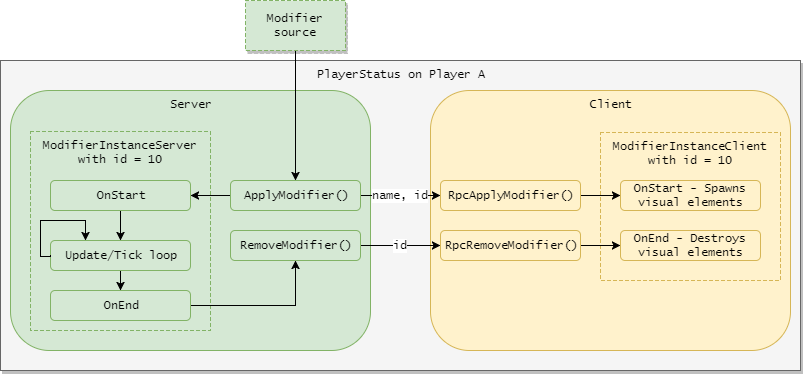
\includegraphics[width=\textwidth]{images/ApplyModifier}
  \caption[Program flow when applying a modifier]{The program flow on Player A when the server applied a modifier.}
  \label{fig:applyModifier}
\end{figure}
 
Figure~\ref{fig:applyModifier} shows the flow when the server applies a modifier to a player. Having two separate instances simplifies the synchronization process, and the server tells the clients to apply a certain modifier by sending the modifier name. However, in cases where multiple modifiers with the same name can be applied we need a way to tell these modifier instances apart other than their name. Otherwise, whenever a modifier effect ends on the server, and it wants to synchronize that to the clients, the client wouldn't know which modifier to remove. By giving a unique id to any modifier applied on the server, it can use that id for both the server and client instance. The
\emph{Modifier} architecture will be described further in Section~\ref{sec:modifiers}.

\section{Modifier architecture}
\label{sec:modifiers}

All modifiers derive from an abstract \emph{Modifier} class. These do not exist as instances, but utilize the \emph{ScriptableObject} class in Unity that is discussed further in Section~\ref{sec:scriptableObjects}. They rely on the \emph{ModifierInstanceServer} and \emph{ModifierInstanceClient} instances to actually run the code present in them. They act more like data containers, and have references to the modifier icon, visual elements and stats. This is why all the functions in the \emph{Modifier} class takes the \emph{PlayerStatus} instance as a parameter, as it can then use that to get references to whichever component on a player it wants to modify, whether it is the player input, or the player object.

The \emph{Modifier} class has quite a few virtual functions, which can be overridden by modifiers depending on what they want to do. They are handled, and called by the modifier instance classes, which means modifiers can be networked through these virtual callbacks. These callbacks are called when the modifier is applied, and when it's removed, with separate functions for the server, local client, and every client. The \emph{ModifierInstanceServer} calls these on the server, in addition to the \emph{OnServerTick} function used for tick loops. And the \emph{ModifierInstanceClient} calls these both for the local client, and every other clients. The code snippet in Listing~\ref{listing:modifierLocalClientStart} is an example of this in the stun modifier, which cancels any abilities being used, and restricts player input.

\begin{listing}[htb]
\begin{minted}[fontsize=\footnotesize]{csharp}
public override void OnLocalClientStart(PlayerStatus playerStatus) {
    playerStatus.GetComponent<Docking>().CancelAbilities();
    playerStatus.GetComponent<PlayerInput>().SetInputRestrictions(...);
}
\end{minted}
\caption[Stun modifier on start]{Code snippet that runs for the local client when the stun modifier is applied.}
\label{listing:modifierLocalClientStart}
\end{listing}


\section{Docking, Docking Kit, and Ability architecture}
These three components are the underlying architecture for the main player gameplay, and are tightly intertwined.

\subsection{Docking}
\label{sec:docking}
The \emph{Docking} component is central to the networking in \emph{Dockit League} and handles the connection between the player and the \emph{DockingKit} component. All networked objects in Unity needs a \emph{NetworkIdentity} component, and these are constrained to root objects.~\cite{unityUNETSpawning} Since the \emph{DockingKit} object is a child of the player object, it can't be networked directly. Our solution to this is therefore to handle all the networking needed for the Docking Kits through the \emph{Docking}. The alternative would be to have the Docking Kit as the root in the scene hierarchy, and either move the entire object position to the owning player each frame, or put the kit visuals as a child of the player. This would keep the \emph{DockingKit} as the root, allowing it to be a \emph{NetworkBehaviour}. However, the same issue would have to be faced for each ability, as they're a child of the docking kit. Having every ability in the root of the scene would lead to a very cluttered scene hierarchy, and way more networked objects than necessary.

\begin{figure}[tbph]
  \centering
  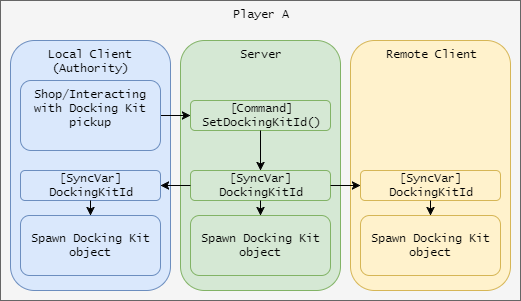
\includegraphics[width=.9\textwidth]{images/CommandSetDockingKit}
  \caption[Program flow on changing docking kit]{The program flow on Player A when the local player changes docking kit.}
  \label{fig:commandSetDockingKit}
\end{figure}

Since the docking kit object itself isn't networked, the clients need to spawn in the object themselves. As shown in Figure~\ref{fig:commandSetDockingKit}, this is initiated by the local client, the player with authority, in this case \emph{Player A}. It's synchronized by passing an enum of the docking kit ID. Keeping this enum as a SyncVar will let the server update this value on every client, a function hook then runs whenever it changes, and updates the representation of \emph{Player A} across every client (and the server) by spawning the object locally.

\subsection{Docking Kit}
The \emph{Docking Kit} was initially the only connector between the abilities and the docking. The abilities only knew the kit it belonged to, and not the docking. However, this lead to a lot of code bloat in the \emph{Docking Kit} that essentially just called a function in the \emph{Docking} component for the abilities. Later this was changed so the abilities have a reference to the \emph{Docking} directly. This reference is set up through an initialization process handled through the \emph{Docking Kit}, which serves its purpose more as a container class for the abilities, and has all it's abilities as children.

\subsection{Ability}
\emph{Ability} is an abstract base class that all abilities inherit from. It has a mix of virtual and abstract functions that can be overridden by abilities if needed. This gives the different abilities flexibility in the way they're implemented. 

\begin{figure}[tbph]
  \centering
  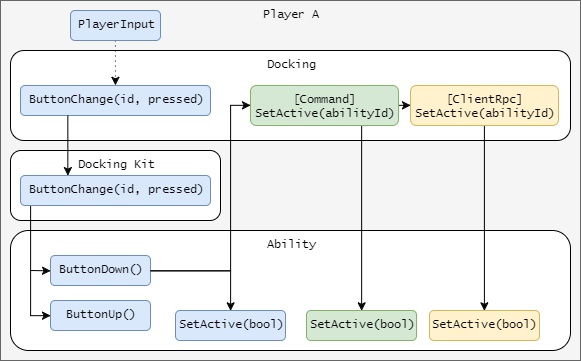
\includegraphics[width=.9\textwidth]{images/CommandSetActive}
  \caption[Program flow on ability button pressed]{The program flow on Player A when the local player presses an ability button.}
  \label{fig:commandSetActive}
\end{figure}

Two of these functions are related to the local player input: \emph{ButtonDown} \& \emph{ButtonUp}. These are called by the \emph{PlayerInput} component, through the \emph{Docking} \& \emph{Docking Kit} whenever an ability button is pressed, along with the ability id, and if the button was pressed or released. This gives no synchronization of the ability, as mentioned in the previous section, that has to go through the Docking. This is shown in Figure~\ref{fig:commandSetActive}, where functions with background color blue, green, and yellow run on the local client, server, and remote clients respectively. In order for the different remote clients to run related ability code, like play animations or sounds for instance, the local client calls \emph{Commands} from the input functions on the docking. The docking then runs the \emph{SetActive(bool)} function on the server, and then uses a \emph{ClientRpc} to run it on every client, except the local client, as that client already ran the function. This means that in the current solution the abilities only have two active states, active or deactivated. This could for instance be expanded to an int, if abilities needed more states.

\begin{figure}[tbph]
  \centering
  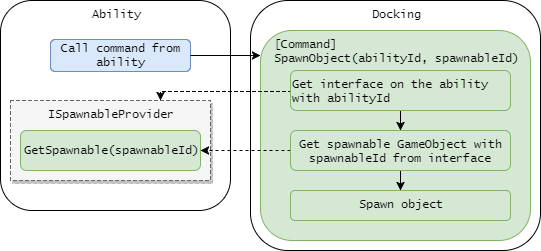
\includegraphics[width=.9\textwidth]{images/SpawnObject}
  \caption[Program flow on ability spawning object]{The program flow when an ability on the local player spawns an object.}
  \label{fig:spawnObject}
\end{figure}

In addition to the virtuals from the base class, abilities can further expand their functionality with interfaces. \emph{ISpawnableProvider} is an interface used if the ability needs to spawn an object. The ability can't handle that itself, because it needs to be networked. A command is called on the docking, but in order for the docking to know which ability called for an object to be spawned, it takes an int as the ability ID. The docking can then get a reference to the ability list through the docking kit, and get the \emph{ISpawnableProvider} interface to call the function that gets the object to be spawned, as seen in Figure~\ref{fig:spawnObject}. This is a necessary step, since the network calls only support basic data types, we can't pass the spawn object reference directly. It allows for the object reference to be held in the ability directly, and the interface allows the docking to get a reference to the correct object when running on the server. In some cases the ability might want to keep a reference to the object spawned. Therefore an additional interface, \emph{ISpawnableReferenceProvider}, and a \emph{Command} \& \emph{TargetRpc} function in the docking was added to allow the server to pass a reference back to the local client. \emph{IModifierProvider} uses the same principles for applying ability modifiers.

These provider interfaces are good for generic functionality in the abilities, but it doesn't give the abilities much flexibility when implementing the gameplay. Therefore additional interfaces were implemented to give the abilities more options: \emph{IServerCallback}, \emph{IClientCallback}, and \emph{ITargetCallback}. These callbacks are tied to the networking attributes \emph{Command}, \emph{ClientRpc}, and \emph{TargetRpc} respectively. This basically gives the abilities a way to be networked without being \emph{NetworkBehaviours}. These interfaces were implemented with generics, to allow different abilities to use different parameters for these callbacks. However, the Unity networking doesn't support generic functions, nor overloading, with these attributes. Therefore, separate functions with different names had to be created in the docking. Unity's networking limitations are discussed further in Section~\ref{sec:networkLimitations}.

\section{Docking Kits}
\label{sec:dockingKits}
This section covers a mix of the final design of the kits as well as well as some more technical details on their abilities. Additional documentation on docking kits can be found in Appendix~\ref{app:doxygen}.

\subsection{Basic Kit}
The Basic Kit is the starter kit, and a kit that's always available for the player. It is the only kit with just one ability, and exists to make sure the player has a kit, in case they can't afford or pick up any other kits.

\begin{figure}[tbph]  %t top, b bottom, p page | you can also use h to try to get the figure to appear at the current location
  \centering
  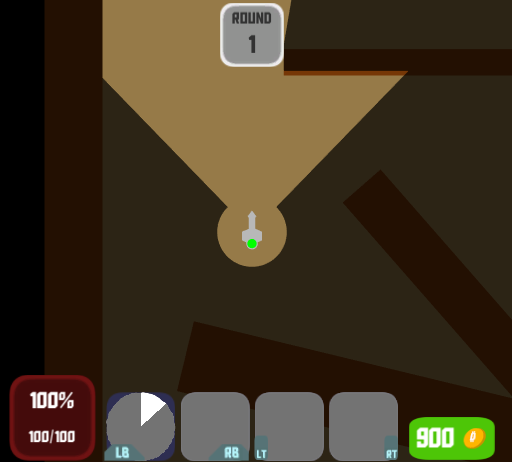
\includegraphics[width=.75\textwidth]{images/BasicAttackActive}
  \caption[Screenshot of Basic Kit]{Showing the Basic Kit with its basic attack active and extended.}
  \label{fig:basicKit}
\end{figure}

\paragraph{Basic Attack}
A forward melee attack with low cooldown and low damage. It extends the little spike in front of the player model to prod enemies and deal damage. Figure \ref{fig:basicKit} illustrates the maximum range of the Basic Attack.

\subsection{Bomber Kit}
\begin{figure}[tbph]  %t top, b bottom, p page | you can also use h to try to get the figure to appear at the current location
  \centering
  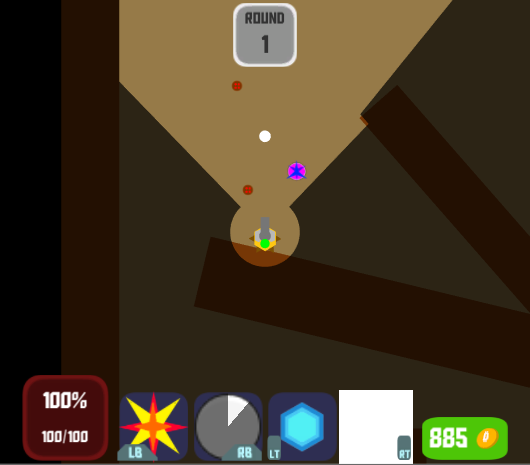
\includegraphics[width=.75\textwidth]{images/BomberKitMinesPlaced}
  \caption[Screenshot of Bomber Kit with mines placed]{what the Bomber Kit looks like in game, with a few of the icons still as placeholders.}
  \label{fig:BomberKitMines}
\end{figure}
The Bomber Kit is a kit based around explosions. It has medium health, low speed and high damage. The abilities of the bomber kit are focused on area of effect damage and knockback to maneuver itself and displace enemies, while also focus on placement and timing for placeable mines. For all the explosions in this kit the damage and knockback is reduced the further away from the explosion the affected unit is.

\paragraph{Explosive Mine}
The first ability is an explosive mine that the player can place, which will trigger when an enemy steps on it. The ability itself uses a script, \emph{ExplosiveMineSpawner}, to spawn and keep a \emph{List<GameObject>} for the mines it spawns. There is a limit of active mines at the same time. When the limit is exceeded, the ability will remove the first mine placed from the list and destroy it. Since each mine handles collision themselves with \emph{OnTriggerEnter}, there was a need to know which mine to remove from the list of active mines. To quickly get a unique ID for the mine, we used \emph{GameObject.GetInstanceID()} at the time of creation and stored this to check the list for which mine to remove in the future. When the mine is triggered by an enemy player, it will start a function \emph{Explode()} which will start an animation and apply forces as well as damage to the players in the area. When the animation ends the mine will destroy itself with an \emph{AnimationEvent} and tell the \emph{ExplosiveMineSpawner} that it's destroyed and should be removed from the list of active mines. Figure \ref{fig:BomberKitMines} shows two mines placed and waiting to trigger.

\paragraph{Grenade Launcher}
The second ability is a grenade launcher. It fires slow, powerful shells that will explode after a certain time or on contact with an enemy. These shells will not explode on contact with the player who fired them, but will deal half the damage to the player when it explodes. They will also bounce off obstacles like walls using a bouncy \emph{Physics Material} added to the shell's \emph{SphereCollider} to make it potentially harder to dodge and master. When the grenade shell explodes, it will check for colliders using \emph{Physics.OverlapSphere} which will return all the colliders in the radius of the sphere created from this. From these colliders the valid targets, self and enemies, will be affected by the explosion. The explosive mine and the grenade shell are much the same in the way they both check for targets with \emph{Physics.OverlapSphere} and apply force with \emph{Rigidbody.AddExplosionForce}. This force is applied by the server to prevent varying results depending on the world state when it gets applied, see Section \ref{sec:conForce} for more on consistent force application.

\paragraph{Remote Mine}
The third ability in this kit is a remote mine that uses much of the same code as the explosive mine, but the main difference here is that you can only have one(1) active at a time and will not trigger on contact. When the player uses this ability again while having a mine active already, it will trigger the remote mine and apply a stun in an area around the mine to all enemies. This ability gives the kit great utility to start a team fight with the proper placement. Like the \emph{Explosive Mine}, this mine gets spawned by the ability using the \emph{ISpawnableReferenceProvider}. This way the ability which spawns the mine will keep a reference to the mine it spawned, and can therefore trigger it when the player activates it a second time. In Figure \ref{fig:BomberKitMines} you can see a purple remote mine placed by the player.

\paragraph{Blast}
The final ability of the Bomber Kit. As the name suggests, it fires a rectangular blast in front of the player that will knock the player backwards, and enemies away. Due to the kit's low movement speed, this ability is a great tool to get out of a bad situation and keeping distance to the enemy. The reason for using a \emph{BoxCollider} instead of something like a cone, is due to the limitation of primitive colliders in Unity3D, briefly explained in Section \ref{sec:updatingGameEngine}. For applying this ability the box collider is disabled until the ability is used. Then it is activated for a frame so the \emph{OnTriggerEnter} function can apply forces before it is disabled again.

\subsection{Boomerang Kit}
The Boomerang Kit is a high speed, high damage kit with low health. The kit's abilities are primarily focused on augmenting the boomerangs that the player can throw. The boomerang itself has a small field of view circle around itself which allows the player to still see the boomerang if it has been thrown across a wall or other areas where vision is limited. 

\begin{figure}[tbph]  %t top, b bottom, p page | you can also use h to try to get the figure to appear at the current location
  \centering
  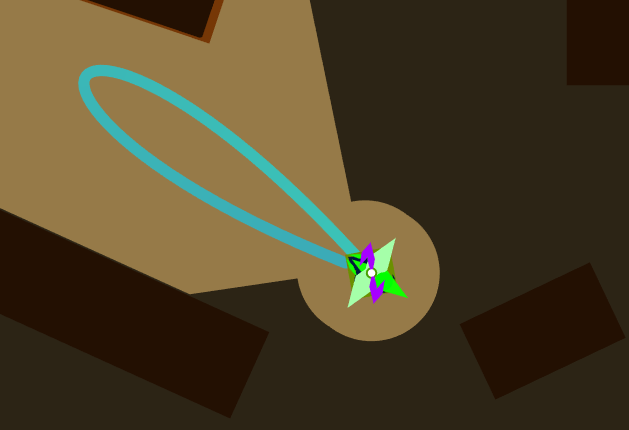
\includegraphics[width=.75\textwidth]{images/boomerangKitLineRenderer}
  \caption[Approximate travel path of the boomerang]{A screenshot from the game showing the approximate travel path of the boomerang when the ability button is held.}
  \label{fig:boomerangLineRenderer}
\end{figure}

\paragraph{Boomerang Throw}
The primary ability of the Boomerang Kit is the boomerang throw. It uses cubic bezier curves to construct and display the approximate path that the boomerang will travel using a \emph{LineRenderer} component. Figure~\ref{fig:boomerangLineRenderer} shows how the approximate path looks like for the local player using the kit. 
The bezier curves are also used for interpolating the position of the boomerang as it is thrown by the player. The interpolation itself is handled using a timer variable that gets updated with \emph{Time.deltaTime} per update loop. The timer is then used as input into an evaluation function used for controlling the speed of the animation and returns a smoothed version of its input. This output is then used as the input time for the bezier curve's interpolation. A more in-depth look at the interpolation of the boomerang throw can be found in Section~\ref{sec:boomerangCurve}. 
    
There are also two additional boomerangs that can be activated with the final ability in the kit. These have their own bezier curve control points and \emph{LineRenderer} components.
In order to perform the same operations on all boomerangs we have a array of structures containing the bezier control points and stored curve handles of each boomerang. This allows us to modify the positions of all the bezier control points directly in the editor which makes it easy to control the shape of the curves.  

\paragraph{Boomerang Root}
The second ability in the kit applies a root modifier to any enemy players within a certain range of the boomerang at the time of activation. It displays a range indicator for the local player whenever the ability is off cooldown, making it easier to time the activation of the ability. Activating the ability will play a short ability animation around the boomerang on all clients and enables the \emph{SphereCollider} component that checks for enemy players. The collider stays active for 0.5 seconds to make it a bit easier for the player using the ability to hit others as the boomerang moves at a fairly high speed. 

\paragraph{Boomerang Vision}
The next ability in the kit is a fairly simple ability that revolves around using a self applied modifier to control the state of its effects. Using the ability takes the \emph{FieldOfView} component of the boomerangs and quickly interpolates the radius of these to a higher value, giving the player a large circle of vision for a short duration. The additional vision is only something the local player can see while other players will see a circle indicator around the boomerang that showcases the new vision range. Once the duration of the modifier runs out the vision range quickly interpolates back to its default value. 

\begin{figure}[tbph]  %t top, b bottom, p page | you can also use h to try to get the figure to appear at the current location
  \centering
  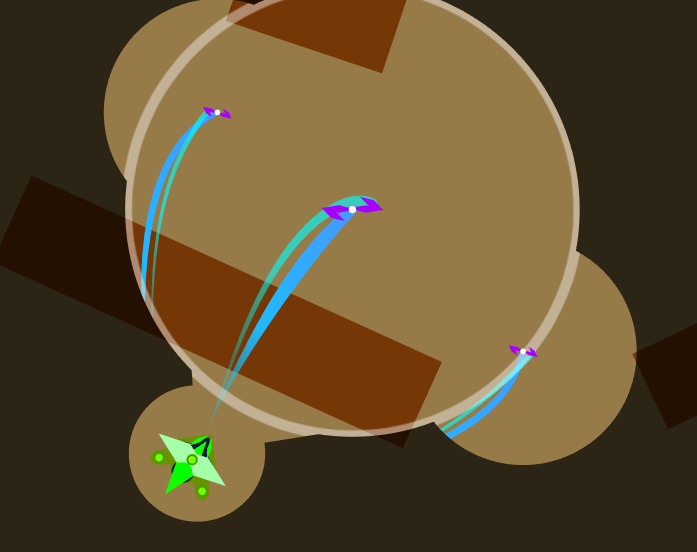
\includegraphics[width=.75\textwidth]{images/boomerangKitMultirang}
  \caption[Screenshot of the multi-boomerang ability]{A screenshot illustrating a player using the final ability of the boomerang kit to throw multiple boomerangs in conjunction with the vision ability.}
  \label{fig:boomerangMultirang}
\end{figure}

\paragraph{Multirangs}
The final ability of the Boomerang Kit is another self applied modifier that lasts for a few seconds and makes the next boomerang throw contain three boomerangs instead of one. This is the key ability of the kit that allows for a truly massive damage output given that the player is able to hit with all of the boomerangs. The self applied modifier is removed prematurely once a boomerang throw is made, but can also wear of naturally if the player avoids throwing any boomerangs during its duration. 

The additional boomerangs granted from this ability are also affected by the root and vision abilities, albeit with a lesser range as seen in Figure~\ref{fig:boomerangMultirang}. The script for the boomerang throw handles the interpolation of the two additional boomerangs while the script for this ability primarily manages the state of the buff. This includes self applying the modifier buff, managing the state of any extra visual elements and playing animations. 


\subsection{Brawler Kit}
The Brawler Kit is a slow moving melee oriented kit, but has high health and multiple tools for dealing with enemies who fight at range. 

\paragraph{Axe Slash}
The first ability is a short cooldown slash with the Brawler Kit's axe. We are using \emph{OnTriggerStay} instead of \emph{OnTriggerEnter} as the collision callback for this ability. This is due to the fact that the animation for the slash is very quick and only lasts a few frames at its start position. Using \emph{OnTriggerEnter} in this case would make the callback frequency too low at the start of the animation, essentially making it impossible to hit players nearby the start position of the axe. This happened because the first few frames would only trigger collision callbacks for the player's own overlapping collider instead of others. 
This issue is alleviated by using \emph{OnTriggerStay} instead with a stored list of hit players. The list is reset after each swing and makes sure that any damage is only applied to each player once. 

\paragraph{Lifesteal}
The second ability in the kit is a self applied modifier that lasts for a certain duration, making the next axe slash deal increased damage and heal a certain percentage of the damage done. It works in a similar fashion to the final ability of the boomerang kit. The self applied modifier can wear off naturally or be removed after colliding with another player. Having the modifier active also changes the visuals of the axe to show that the ability has been used. 

\paragraph{Projectile Reflect}
The third ability is a self applied modifier that reflects the velocity of any projectiles that hits the player while active. This is handled using C\# interfaces. Any projectile that is reflectable needs to implement the \emph{IReflectable} interface. This in turn allows the ability to check whether the interface exists on any colliding projectiles and ask them to reflect their velocity. The ability itself does not perform any reflection directly as this is what the projectiles implementing the interface have to contain.

\begin{figure}[tbph]  %t top, b bottom, p page | you can also use h to try to get the figure to appear at the current location
  \centering
  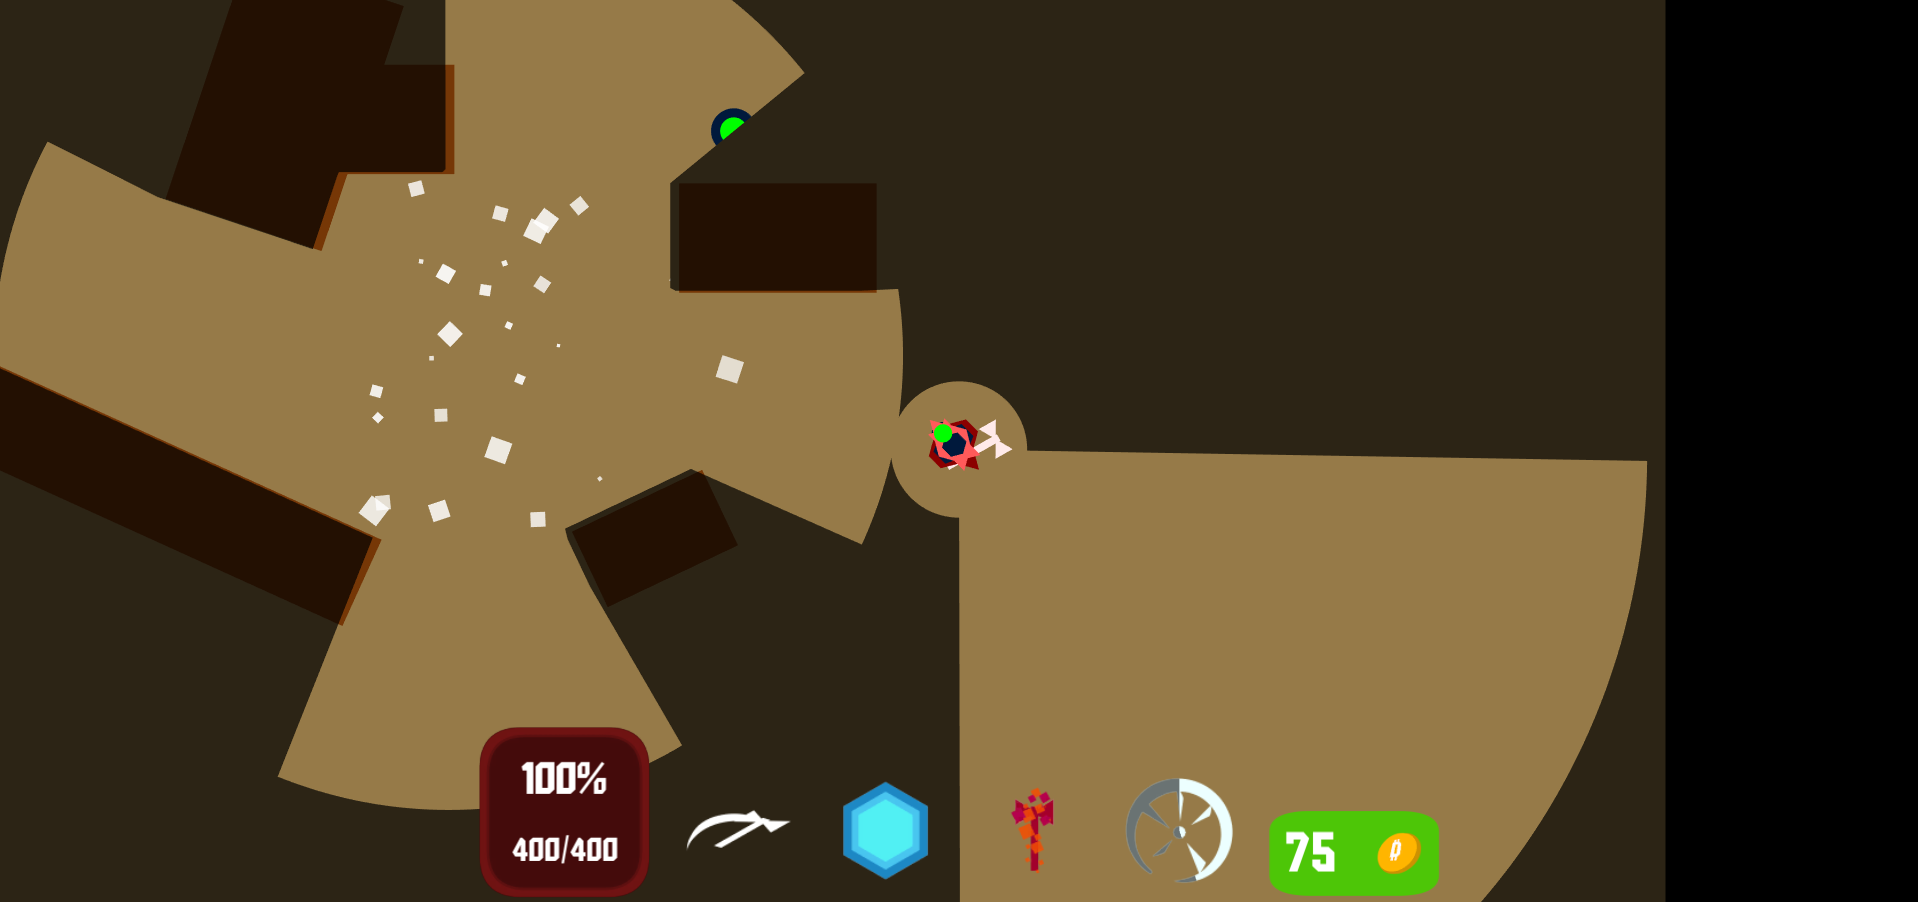
\includegraphics[width=\textwidth]{images/stunGrenade}
  \caption[Screenshot of the brawler kit's stun grenade]{A screenshot from the game showcasing the additional vision range granted from an exploded stun grenade}
  \label{fig:brawlerStunGrenade}
\end{figure}

\paragraph{Stun Grenade}
The final ability makes the player throw a stun grenade that explodes after a short while, providing temporary vision for all players(see Figure~\ref{fig:brawlerStunGrenade}) and applying a stun modifier to anyone looking towards the explosion center. The grenade itself is a \emph{SpawnableObject} and controls the application of modifiers, the temporary vision and any visual elements related to the grenade. The player on the other hand has a simple script that handles the spawning of the grenade. The grenade enables a large sphere collider on explosion which checks for any players within its range. A raycast is then used in conjunction with a dot product to check for players looking towards the center of the explosion. Players with obstacles between themselves and the explosion center will not get stunned as the raycast check will end up failing. 

\subsection{Marksman Kit}

\begin{figure}[tbph]  %t top, b bottom, p page | you can also use h to try to get the figure to appear at the current location
  \centering
  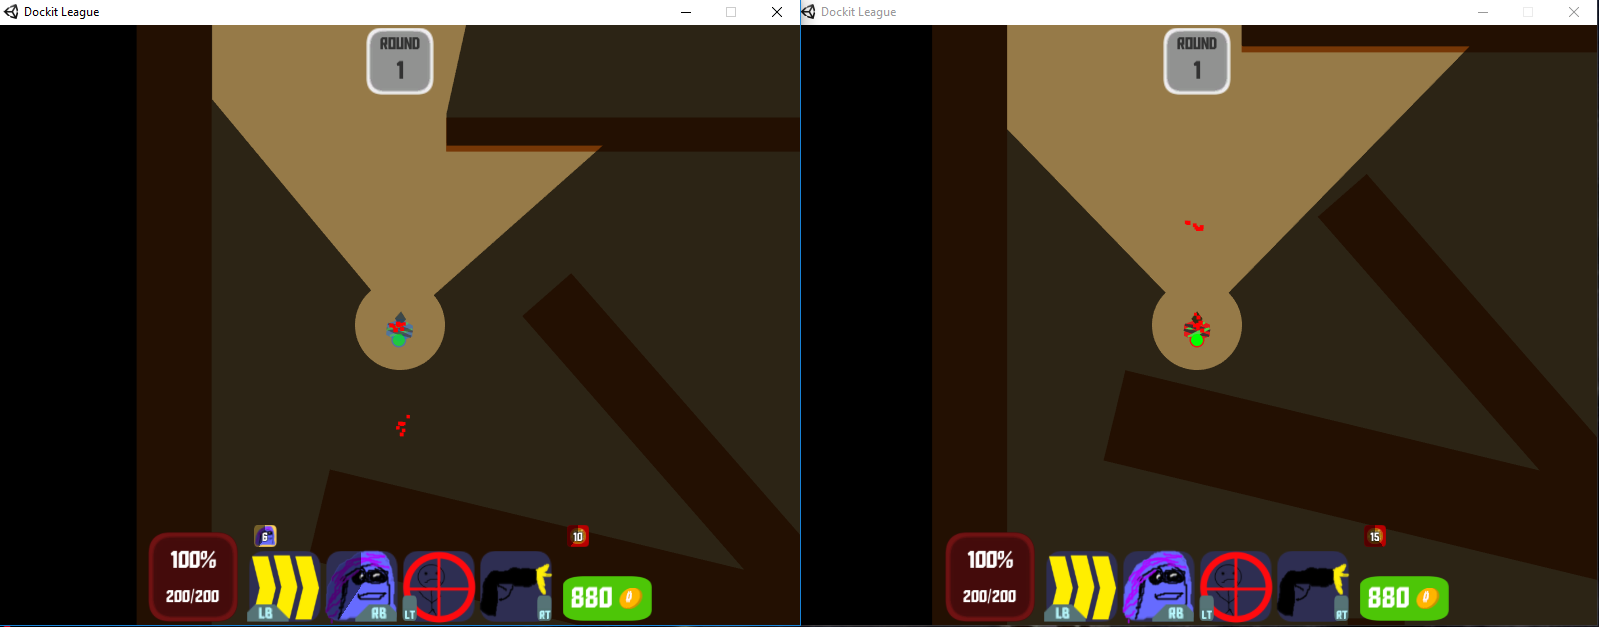
\includegraphics[width=\textwidth]{images/MarksmanKit}
  \caption[Screenshot of Marksman Kit for both teams]{Demonstrates how the stealth and track abilities works, attaching red particles to the player showing the location through fog of war.}
  \label{fig:marksmanKit}
\end{figure}

The Marksman Kit's main focus is to gather information and being elusive to the enemy. With a toolkit that allows it to quickly dash out of harms way, turn invisible and give information about the other team, it is able to give your team the upper hand in a fight. It has medium health, damage, utility and speed, but in the right hands has the potential to be a powerful kit if not dealt with. After playtesting it is worth mentioning that this kit will be renamed later to fit its purpose better.

\paragraph{Dash}
The first ability is the dash ability. A short cooldown ability that applies a small amount of force in the direction you're moving. Since the \emph{PlayerInput} script already has this direction vector stored for player movement, we're simply retrieving the direction from there.

\paragraph{Stealth}
Next up is the stealth ability. This ability lets the player hide its visuals from other players by changing the alpha value to zero. To give it a short fade time, a \emph{coroutine} using a \emph{for-loop} decreases the alpha value over time while accounting for fade time. Stealth can only be broken by using the ability again, fire the projectile ability of the Marksman Kit or when the duration runs out. There was a decision made to not break out of stealth upon taking damage, which is a game mechanic we see often related to stealth or invisibility in games. Therefore the balance around the up-time and frequency of which you can use the ability is important when there is no real way to force the player out of stealth. While in stealth the player also benefits from the stealth modifier. This is a modifier that amplifies the Marksman Kit's next projectile shot from stealth, boosting damage while applying a slow and silence to an enemy if it hits. This is applied to the \emph{projectile} fired when the projectile is initialized, giving it a reference to the stealth buff that applied it with the data of the buff.

\paragraph{Track}
This ability is a tracking debuff the Marksman Kit can apply to enemies. It will then reveal the position of the marked player while amplifying the damage taken from all sources, see Figure \ref{fig:marksmanKit}. To apply this debuff the player fires in a straight line in front of him with a \emph{Physics.RaycastAll} and applies it to the first player it hits that isn't covered by an obstacle. We could potentially have done this differently by using \emph{Layers} in Unity to filter out which game objects should be ignored from raycasts and not. Although \emph{Physics.RaycastAll} doesn't guarantee a sorted order, all \emph{RaycastHit} have a variable \emph{distance} from the point of impact to the origin of the raycast which we can sort with a lambda. Listing \ref{listing:applyingTrack} shows how this is sorted and applied to the first enemy hit that isn't covered.

\begin{listing}[htb]
\begin{minted}[fontsize=\footnotesize]{csharp}
void IServerCallback.ServerCallback(int functionId) {
    var hits = Physics.RaycastAll(transform.position, transform.forward, castRange)
                    .OrderBy(h => h.distance);
    
    foreach(RaycastHit hit in hits) {
        if (hit.collider != null && hit.collider.CompareTag("Obstacle")) {
            return;
        }
        if (hit.collider != null && 
            this.docking.CheckDamagable(hit.collider.GetComponent<Player>())) {
            
            PlayerStatus playerStatus = hit.collider.GetComponent<PlayerStatus>();
            if (playerStatus != null) {
                playerStatus.ApplyModifier(trackInfo);
                return;
            }
        }
    } 
}
\end{minted}
\caption[Applying the tracking debuff]{Code snippet for applying Track to first enemy not behind an obstacle.}
\label{listing:applyingTrack}
\end{listing}

\paragraph{Projectile}
Finally we have the last ability we simply called Projectile. It is a basic "fire in a straight line"-type of projectile, and it is the only source for this kit to deal damage directly with. It has an \emph{Ability} script \emph{ProjectileSpawner} which instantiates projectile prefabs and \emph{Initialize} them with the stealth buff reference and a \emph{Boolean} indicating if it's active. Each projectile has its own lifetime, destroying itself after a while if it doesn't hit any players or obstacles. For physics we've chosen to not have a constant velocity, but rather apply \emph{Impulse Force} when the projectile is fired for this. This worked fine when we tested it in the editor, but after playtesting it proved that the projectile would lag, unlike the projectile from the Sniper Kit. Therefore this is a change to be made to use the \emph{Transform} instead of the \emph{Rigidbody} to move the projectile.

\subsection{Sniper Kit}
The Sniper Kit is the long range focused kit. Keeping your distance gives you time to charge, which is important with varying damage output and precision depending on charge time.

\paragraph{Shackle}
The first ability is Shackle, which launches a bola that travels a short distance before disappearing. It is designed to give the player in this kit a way to get away from enemies getting close, since staying at range is beneficial. If the bola collides with an enemy player it has three different outcomes depending on the scenario. If there is nothing behind the player hit, it will apply a slow modifier. If there is an obstacle behind them, the stun modifier is applied instead. And the third option is if there is another enemy player behind the first one hit, they're both stunned. This is done by firing a raycast from the center of the player hit, in the direction the bola was travelling. If this doesn't hit anything, we can apply the slow. If it hits something, we first check if it's an obstacle, if so we apply the stun. If it's not a wall, we can check if it's another player, and stun both of them if that's the case. The three outcomes are shown in Figure~\ref{fig:shackleOutcomes}.

\begin{figure}[htbp]  %t top, b bottom, p page | you can also use h to try to get the figure to appear at the current location
  \centering
  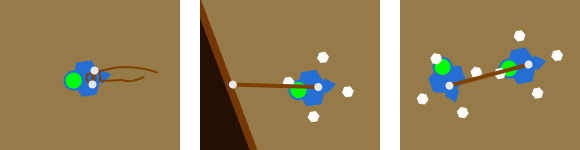
\includegraphics[width=\textwidth]{images/ShackleOutcomes}
  \caption[Shackle outcomes]{Three screenshots from the game showing the slow, stun against wall, and stun against another player from left to right respectively.}
  \label{fig:shackleOutcomes}
\end{figure}

\paragraph{Focus}
The second ability is Focus, and is more of a utility ability used in addition to the Slingshot ability. It will root the player in place, and increase the line of sight distance, but decrease the view angle using the lerp functionality in the \emph{FieldOfView} script for a smooth transition. It will also move the camera forward slightly with a similar functionality in the \emph{PlayerCamera} script. The use of this is displayed by moving the sling mounting forward, and retracting the sling.

\paragraph{Slingshot}
The third ability is Slingshot, and the damage ability for this kit. On button press it starts charging the slingshot precision, starting at the view angle and moving towards 0 using an animation curve. The ability uses a different curve for the initial charge towards 0, and a hold curve that reduces the charge angle back to the view angle over a few seconds after reaching max precision, preventing the player to keep max precision for a long time. When the button is released it will fire a projectile at a random angle between the charge angles, meaning the smaller the charge angle is, the more precise it'll be. The projectile damage, speed, and lifetime depends on both the fire angle and the charge angle, which means that two projectiles fired at the same angle might have different stats depending on the charge time. This is simply to make sure a charged attack will always do more damage than a lucky shot with no charge. The ability mid-charge is shown in Figure~\ref{fig:slingshotCharge} where the white lines represents the charge angles.

\begin{figure}[htbp]  %t top, b bottom, p page | you can also use h to try to get the figure to appear at the current location
  \centering
  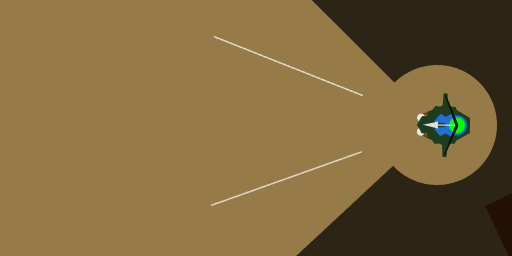
\includegraphics[width=\textwidth]{images/SlingshotCharge}
  \caption[Slingshot charge]{A screenshot from the game showing the Slingshot ability mid-charge.}
  \label{fig:slingshotCharge}
\end{figure}

\paragraph{Zipline Gun}
The final ability is the Zipline Gun, and like Shackle, it's a way to get away from enemies by setting up an escape route for when a situation gets rough, or just quickly move to another vantage point. This ability has two different states, the first is the initial state, when nothing has been fired. When used in this state a zipline object is spawned on the server, and the server side of the ability keeps a reference to that object. The second state is when we've already set up the first zipline point, we then fire the second point to complete the zipline. There are a few restrictions when setting up the zipline, and it needs to constantly check if any of these are broken. Initially, when we fire a point it needs to hit an obstacle, this is checked by firing a raycast in the direction, with the given range, the zipline is fired. If this is anything other than an obstacle or out of range, the zipline setup is invalid, and the zipline object is destroyed. After firing the first point, a \emph{Coroutine} is started that keeps checking if there is anything interfering the zipline by firing raycasts between the player and the first point. When firing the second point, this check fires between the first and the second point instead, preventing setting up ziplines that cuts across a corner for instance. Figure~\ref{fig:ziplineMidSetup} shows the kit between the first and the second state, and areas where a setup is invalid.

\begin{figure}[htbp]  %t top, b bottom, p page | you can also use h to try to get the figure to appear at the current location
  \centering
  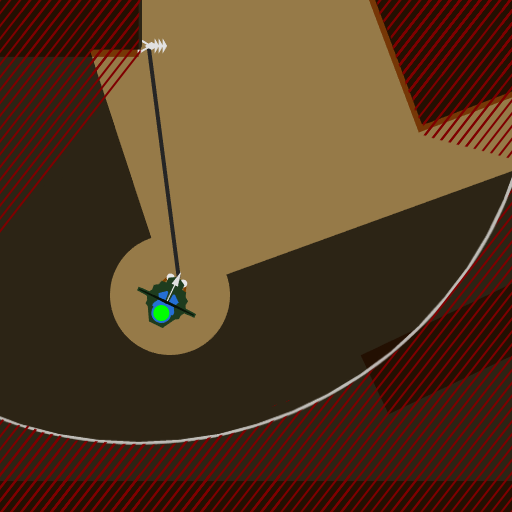
\includegraphics[width=.6\textwidth]{images/ZiplineMidSetup}
  \caption[Zipline mid-setup]{Showing the state between the first and second point fired, with invalid areas covered. (Red lines are not present in-game)}
  \label{fig:ziplineMidSetup}
\end{figure}

\subsection{Tank Kit}
The Tank Kit's purpose is being the front line for the team, having a lot of health allows it to soak up the damage dished out by enemies by redirecting projectiles. It is a very slow kit, but compensates by having abilities for pulling both itself and others around.

\paragraph{Reflect Shield}
The first ability is Reflect Shield. This is a shield that can be activated, and will stay active for a certain duration. Any object colliding with this shield that implements the \emph{IRedirectable} interface will be redirected, and the Tank Kit player will take ownership of the object redirected. The new direction of the object is the same direction as the Tank Kit player is facing. This is done using the \emph{OnTriggerEnter} callback, and getting the interface from the object passed in. An object is restricted to only be redirected once per ability use, this is handled by adding any redirected objects to a list, and simply checking if the list already contains the object that's to be redirected. This list is then cleared when the ability is deactivated.

\paragraph{Force Field}
The second ability is Force Field. While the Reflect Shield is all about moving things away, the Force Field is about pulling things in. This also affects objects with the \emph{IRedirectable} interface, and the implementation of that part of this ability is similar to the Reflect Shield. However, this ability redirects object towards yourself, and doesn't take ownership of the object, meaning the Tank Kit player will take damage from the objects pulled in. Here the synergy with the Reflect Shield comes to fruition, as the shield can reflect objects pulled in by the field. In addition to pulling objects in, this ability also pulls in other players, compensating for the lack of movement speed, as well as synergizing with the Power Saw. This is also handled in the \emph{OnTriggerEnter} callback, and calls one of the \emph{TargetRpc} function in the player for adding force. The implementation of those are discussed in Section~\ref{sec:conForce}.

\paragraph{Power Saw}
The third ability is the Power Saw. This has two stages, the initial state is a wind-up for the release of the sawblades. This will do damage to enemy players coming in contact with the sawblades, using the \emph{OnTriggerEnter} callback. To prevent players being hit multiple times consecutively, they're added to a list the first time hit. If the callback triggers on a player, it only does damage if the player isn't already in the list. This list is then cleared when the swing is completed. When the wind-up state is complete the sawblades are released. At this point they're spawned in as actual objects by the local client calling a command on the \emph{Docking} script, which spawns the object on the server. The cooldown on this ability can be reduced by picking up sawblades that has come to a halt. This is handled by the \emph{Sawblade} script, which is a component on the sawblade object spawned. If an object with a \emph{Docking} component enters its trigger, it will retrieve all the abilities, and check if any of the abilities is of the type \emph{PowerSaw}. If so reduce the cooldown of that ability through the docking, and delete the sawblade object, as shown in Listing~\ref{listing:sawbladesPickup}.


\begin{listing}[htb]
\begin{minted}[fontsize=\footnotesize]{csharp}
for(int i = 0; i < dockingKit.abilities.Count; i++) {
    if(dockingKit.abilities[i] is PowerSaw) {
        docking.TargetReduceCooldown(..., i);
        NetworkServer.Destroy(gameObject);
        break;
    }
}
\end{minted}
\caption[Check on sawblade pickup]{Code snippet for checking if the player trying to pick up the sawblade has the PowerSaw ability.}
\label{listing:sawbladesPickup}
\end{listing}

By using a \emph{for} loop here, we can use the iterator count as a parameter to the reduce cooldown function in the docking, that way the docking knows which ability to reduce the cooldown for without the need to specify it anywhere, and having to manually update it if the ability order is reordered.

\paragraph{Hook Shot}
The final ability is the Hook Shot, which fires out a hook when used. Whenever the hook hits an obstacle, or a player, it will pull the Tank Kit player towards the point the hook connected with its target. If the hook hits an enemy player it will also apply a root to that player. The hook animation is handled locally by every client, and is in this case animated by the script. The ability utilizes both the \emph{IServerCallback and }\emph{IClientCallback} interface. The server callback is for launching the hook, and passes along two \emph{Vector3}: The launch position, and launch direction. The server then uses the client callbacks to pass these to every client, allowing them to replicate the hook animation as precisely as possible. The reason for this is that the hook is launched in the player forward direction, and the player rotation on the server and rotation on the local client isn't necessarily the exact same, especially when a player rotates as they're triggering the ability. 

The server can't simply launch the hook forward, because the forward direction the player had when they triggered it, isn't the forward direction when the server receives the trigger message. The hit registration is handled by the server, which will use callbacks to let the clients know what to do. The default behaviour is to extend the hook to max range, and then retract it. This is what the clients will do as long as the server doesn't tell them otherwise. If the hook hits an obstacle or a player the server will tell the clients to freeze the hook in a certain position for a moment, before retracting. The hook can also hook certain objects, like the sawblades. The sawblades implements the \emph{IHookable} interface, which is used in the \emph{OnTriggerEnter} callback in the Hook Shot. This allows the Hook Shot to be used for picking up sawblades without actually moving to them.

\subsection{Trapper Kit}
The Trapper Kit is a utility docking kit that focuses on using its three traps to provide various types of crowd control as well as being adequately capable of fighting enemies in close to mid range using the kit's flamethrower.  

\paragraph{Flamethrower}
The first ability in the kit is the flamethrower, a self applied modifier that activates a large sphere collider that checks for objects that it can burn. One of the limitations of working with Unity3D rather than Unity2D is that we don't have access to polygon colliders. Using polygon colliders would have made it possible to create a cone collider for this ability. We are instead using a large sphere collider for the flamethrower although its shape is not necessarily as fitting.
The collision callback checks for any enemy players and applies a burn modifier to these. It also checks for game objects with the \emph{IElement} interface and applies a fire element to any such objects if found. This means that abilities from other kits that support elemental modifiers can be buffed by the flamethrower.

\paragraph{Trap Overview}
The three other abilities use traps deriving from a base \emph{Trap} class. A shared \emph{TrapSpawner} script is used to spawn each of the three traps by providing it with different prefabs per ability. 
The \emph{TrapSpawner} script handles spawning its given trap prefab as well as updating the visuals of the docking kit to reflect that traps have been placed. Each trap has its own visual element on the docking kit that is modified to allow other players to know which traps the user currently has placed. Figure~\ref{fig:trapperKit} showcases these.
The trap spawner script contains a reference to the spawned trap while the spawned trap is provided with a reference back to its owner. This allows the trap to only stay visible for its owner as well as communicating back to its owner whenever it has been triggered. 

Acquiring the reference to the traps is handled by implementing the \emph{ISpawnableReferenceProvider} interface. Only one trap of each type can be placed at a time so trying to replace a trap that already is placed destroys the old trap and places a new one at the player's current position.  

\begin{figure}[tbph]  %t top, b bottom, p page | you can also use h to try to get the figure to appear at the current location
  \centering
  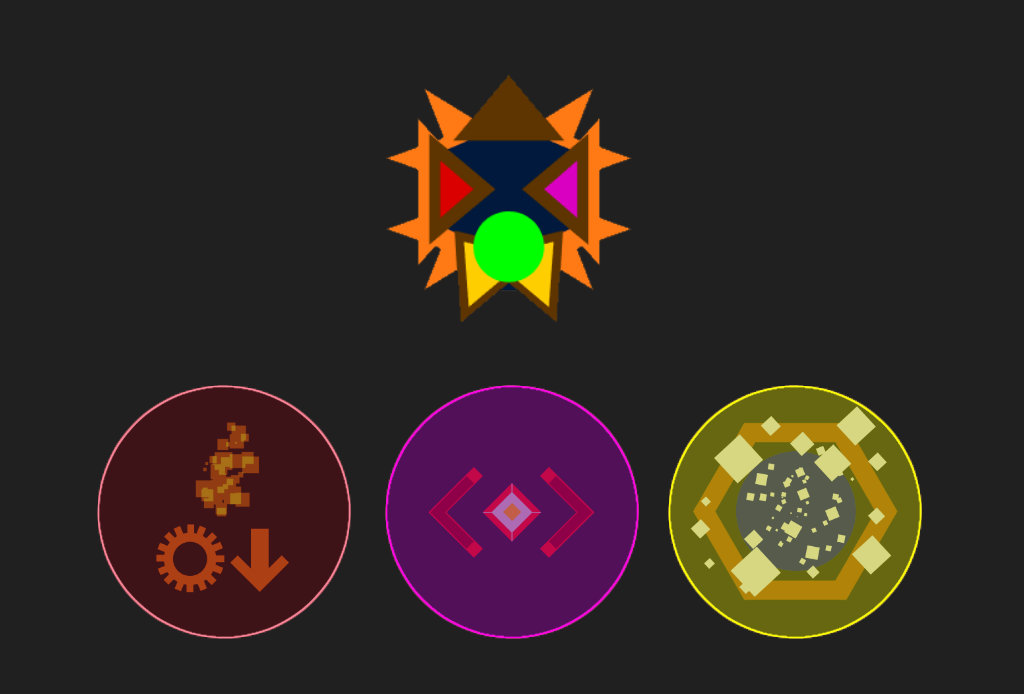
\includegraphics[width=.75\textwidth]{images/TrapperKitWithTraps}
  \caption[The trapper kit with its three traps]{The trapper kit has three traps. Placing one trap fades the color of its associated visual element on the docking kit}
  \label{fig:trapperKit}
\end{figure}

The \emph{Trap} base class handles generic functionality like changing the visual state of the trap to invisible for other players as well as playing animations whenever the trap is triggered. A virtual function is used to allow any children of the base class to provide custom behaviour as the trap is triggered. The base class also contains a list of players that triggered it to make sure that no modifiers are applied twice in the case that a player quickly moves in and out of the trap collider. 

\paragraph{The Slow Burn Trap and the Blind Trap}
The first two traps have fairly simple behaviour. Both have modifiers that they apply to the list of players who triggered the trap. The first applies a burn and slow modifier while the second applies a blind modifier. 

\begin{figure}[tbph]  %t top, b bottom, p page | you can also use h to try to get the figure to appear at the current location
  \centering
  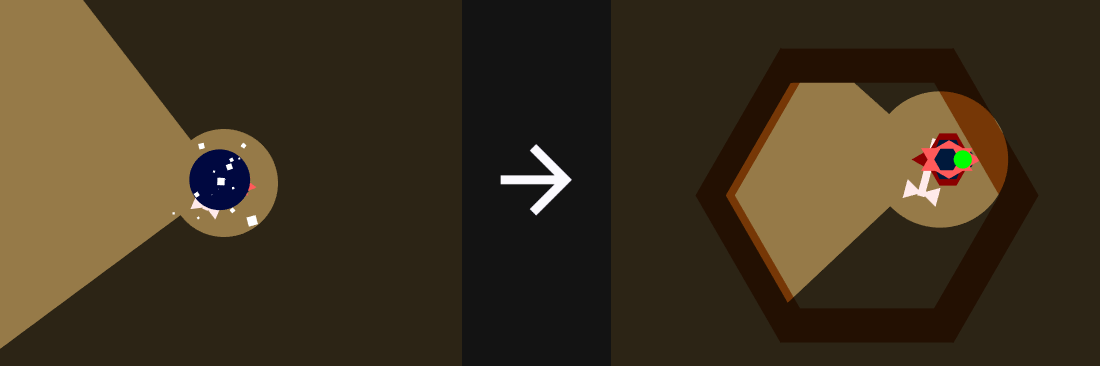
\includegraphics[width=\textwidth]{images/trapperKitCaptureTrap}
  \caption[Two screenshots showing off capture trap of the trapper kit]{These two screenshots show the two main stages of the capture trap's life cycle.}
  \label{fig:trapperKitCapture}
\end{figure}

\paragraph{The Capture Trap}
The third trap has more custom behaviour compared to the previous two. It pulls in any nearby enemy players after triggering and places a temporary wall around these players to "capture" them for a short duration as seen in Figure~\ref{fig:trapperKitCapture}. There are a lot of different visual elements like particle systems, animations, colliders and sprites that are enabled/disabled throughout the trap's lifecycle. 

Applying the force for pulling players into the trap is done using a \emph{TargetRpc} function located in the main player script while a C\# coroutine is used to enable the walls after a short duration. More information on adding consistent force to both the server and clients can be found in Section~\ref{sec:conForce}. 

\subsection{Support Kit}
The Support Kit is a kit made to keep your team alive. It is centered around just staying alive with your team, healing them over time while slowly draining your enemies of their lives. The kit have medium health and speed to make it fairly hard to kill, while being able to negate damage and remove debuffs further increasing its sustainability.

\begin{figure}[tbph]  %t top, b bottom, p page | you can also use h to try to get the figure to appear at the current location
  \centering
  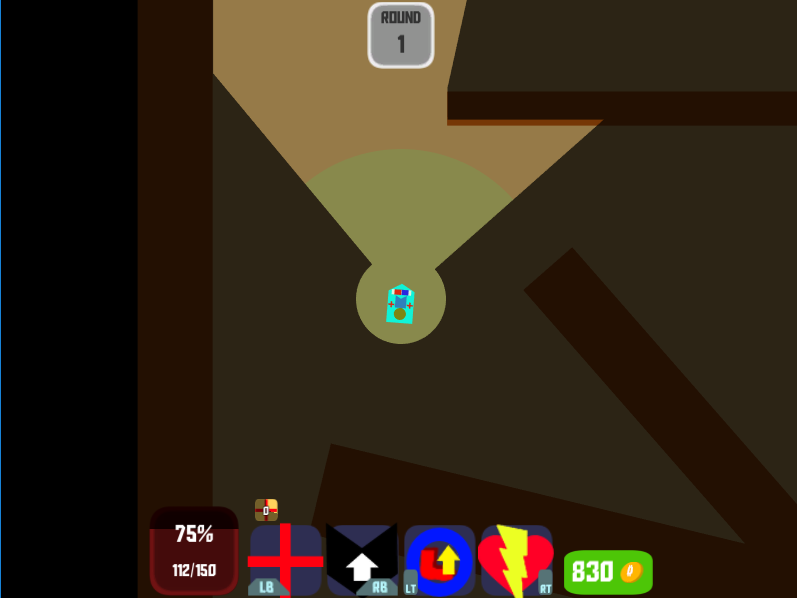
\includegraphics[width=\textwidth]{images/SupportKitHealing}
  \caption[Screenshot of the Support Kit]{Shows the Support Kit with healing aura toggled on.}
  \label{fig:supportKit}
\end{figure}

\paragraph{Healing Aura}
The first ability in the Support Kit. This aura applies healing in a circle around the player that can be toggled on and off, see the green circle in Figure \ref{fig:supportKit}. It uses a \emph{List} to keep track of players in the aura, and this list updates whenever players enters and exits the aura. Using the \emph{IServerCallback} interface, the healing aura applies a buff to the players every healing-interval to that will heal them. This script also has a reference to the second ability of the kit, the Fortification Buff, which also gets applied here at the same time, strengthening the power of the healing aura.

\paragraph{Fortification Buff}
This is a power-up to the Healing Aura. The buff received from this makes players affected by the Healing Aura take reduced damage. Unlike the Healing Aura, this is a lingering buff that lasts for a few seconds after leaving the area as well. Gives the kit a better tool against burst-damage when used correctly.

\paragraph{Cleanse}
This ability will emit a ring of pure energy, cleansing friendly players hit of any debuff they might have and giving a slight move speed buff for a short amount of time. As mentioned before, Unity3D has a limited selection of primitive colliders, but for this ability we made a ring collider using \emph{Blender}, an open source 3D creation suite. When used, an animation plays that enables the collider and  takes the \emph{Scale} of the \emph{Transform} to make it look like the ring expands. Figure \ref{fig:cleanseAbility} demonstrates what this looks like in game.

\begin{figure}[tbph]  %t top, b bottom, p page | you can also use h to try to get the figure to appear at the current location
  \centering
  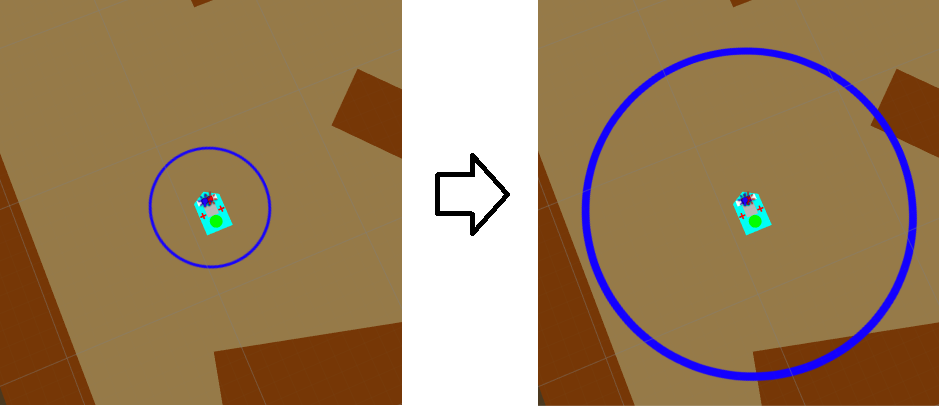
\includegraphics[width=\textwidth]{images/CleanseAbility}
  \caption[Screenshot of the Cleanse Ability from the editor]{Screenshot of the Cleanse Ability in the editor, showing the covered area.}
  \label{fig:cleanseAbility}
\end{figure}


\paragraph{Health Drain}
The only damaging ability of the Support Kit, draining the life of enemies around you and distributing the health drained to teammates around you. The more enemies drained, the more healing to distribute. The More allies, the less healing each ally get. For the time being we are using this simple way of doing it, in the future it should also make sure to check how much health each player loses and heals and take this into account when distributing the healing. Some variables have their names replaced to fit the page:

\begin{listing}[htb]
\begin{minted}[fontsize=\footnotesize]{csharp}
foreach (GameObject player in friendlyPlayersInAura) {
    float healthToHeal = (baseDrain * hostilePlayersInAura.Count) / friendlyPlayersInAura.Count;
    player.GetComponent<PlayerHealth>().Heal(healthToHeal);
}
\end{minted}
\caption[Health Drain distributing health]{Code snippet for distributing the health drained to players around.}
\label{listing:supportHealthDrain}
\end{listing}

\section{Shop Architecture}
\subsection{Visual Layout}
\begin{figure}[tbph]  %t top, b bottom, p page | you can also use h to try to get the figure to appear at the current location
  \centering
  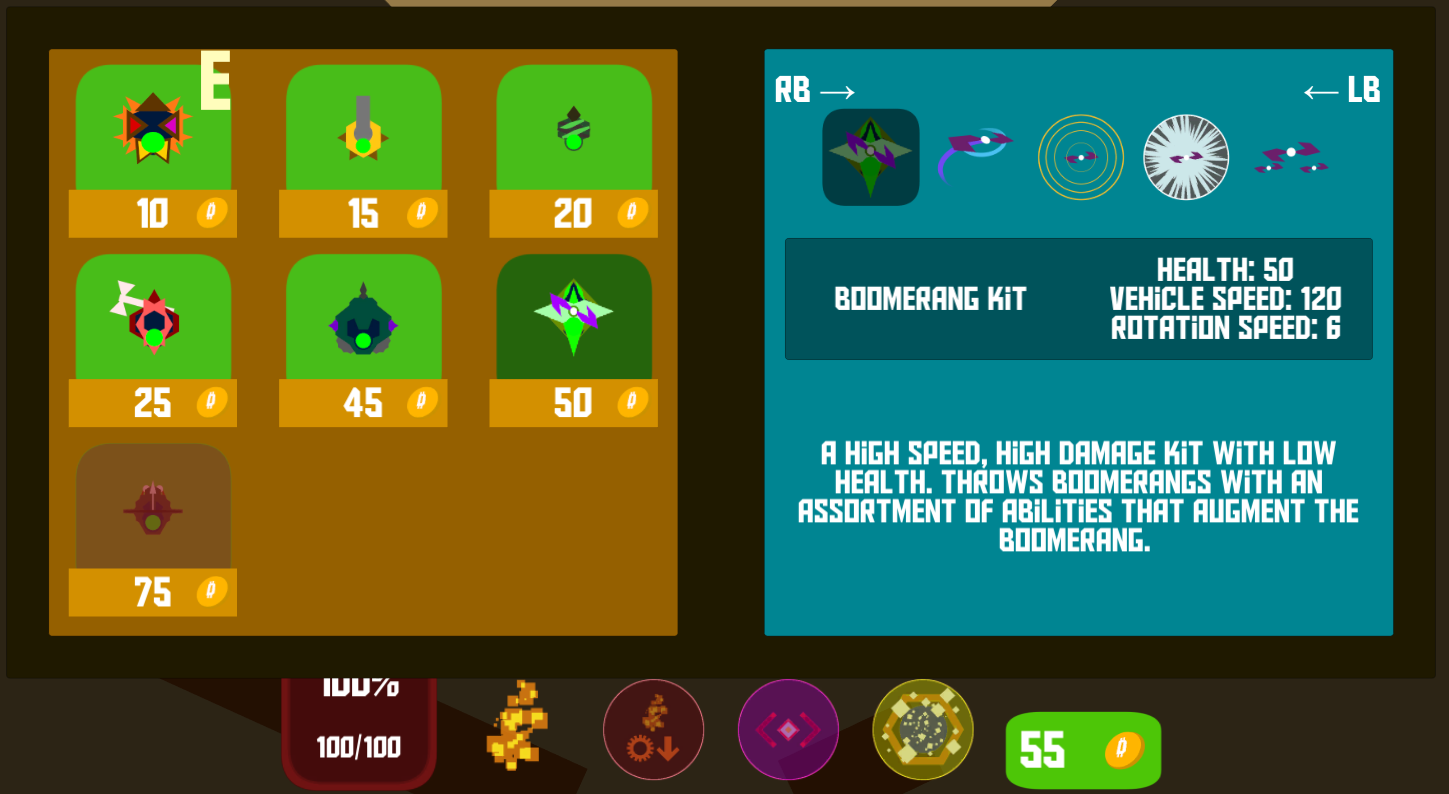
\includegraphics[width=.75\textwidth]{images/shopOverview}
  \caption[Screenshot showing off the in-game shop]{A screenshot showing off the in-game shop}
  \label{fig:shopOverview}
\end{figure}

The visual layout of the shop can be seen in Figure~\ref{fig:shopOverview}. The layout itself is split into two halves. 
The left half contains purchasable shop items while the right half contains individual information on the currently selected shop item. The currently equipped docking kit is signified by a "E" while any unpurchasable docking kits due to lack of currency are greyed out. 
The information display on the right side contains several text boxes that scripts can use to display arbitrary information about the shop item like names, descriptions and additional stats. Each docking kit contains information on the kit and its abilities which is split into five different "tabs". The information tabs for each item can be cycled through by pressing the left and right shoulder buttons on the controller as displayed on the top of the panel.

\subsection{Scriptable objects for shop items}
\label{sec:scriptableObjectsShop}
Scriptable objects provide an easy to use interface for developers, especially if used as described in Section~\ref{sec:scriptableObjects}. It allows us to simply go the the correct resource folder, right click and choose "New shop item". We can then directly fill in any data related to the new shop item in the inspector as seen in Figure~\ref{fig:scriptableObjectInspectorShop}. 
The scriptable object for shop items contains several pieces of data:
\begin{itemize}
    \item The name of the docking kit.
    \item The sprite that is displayed in the left panel of the shop.
    \item The prefab for the related docking kit.
    \item The price of the docking kit
    \item An enum which we use as a ID to identify the docking kit.
    \item A list of structures containing description data. These structures include the sprites used for the tabs on the right panel of the shop, the name of the ability/kit and a description. 
\end{itemize}

The scriptable object itself does not contain any code and is used as a data container. The data within the scriptable objects are then loaded by the menu handler and attached to instantiated shop item instances. 

\begin{figure}[tbph]
  \centering
  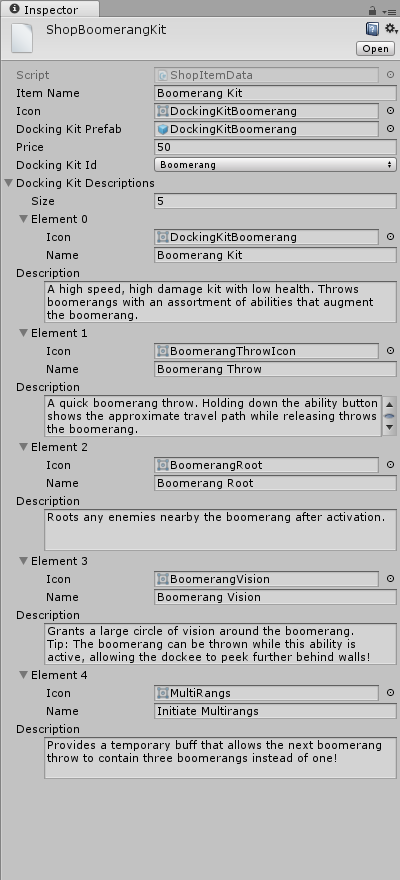
\includegraphics[width=.6\textwidth]{images/scriptableObjectInspector}
  \caption[Image of the Unity inspector showing scriptable objects from the shop]{An image of the Unity inspector that illustrates how one of the scriptable objects from the shop looks like}
  \label{fig:scriptableObjectInspectorShop}
\end{figure}

\subsection{Internal shop management}
The shop architecture in \emph{Dockit League} is split up into several components:
\begin{itemize}
    \item A script, \emph{IngameMenuHandler} manages the shop and any interaction with it.
    \item Scriptable Objects are used to contain data related to the individual shop items. 
    \item Each item instance in the shop contains the \emph{ShopItemInstance script} which stores a scriptable object and handles the data display for it. 
\end{itemize}

The \emph{IngameMenuHandler} script starts by loading all scriptable objects within the project that contain item data. These scriptable objects are then placed in a list and sorted by price before the script starts instantiating \emph{ShopItemInstance}'s with a respective scriptable object. 
The script also handles input for scrolling through the information tabs of the currently selected shop item. This is handled by incrementing and decrementing a range limited integer which is used as a index to access the correct descriptions from the scriptable object. 

We use a prefab with uninitialized visual elements and a \emph{ShopItemInstance} script to spawn in individual shop items. After being spawned, the instance is then initialized by passing a scriptable object over to it and updating all of its visual elements with the acquired data. The \emph{ShopItemInstance} script also contains a callback for whenever it is pressed which displays a purchase verification prompt with a "yes" and "no" answer. Answering "yes" to the prompt tells \emph{IngameMenuHandler} to complete the purchase and equips the new docking kit to the player.  